
\begin{figure*}
  \centering

\begin{subfigure}[b]{\textwidth}
\centering
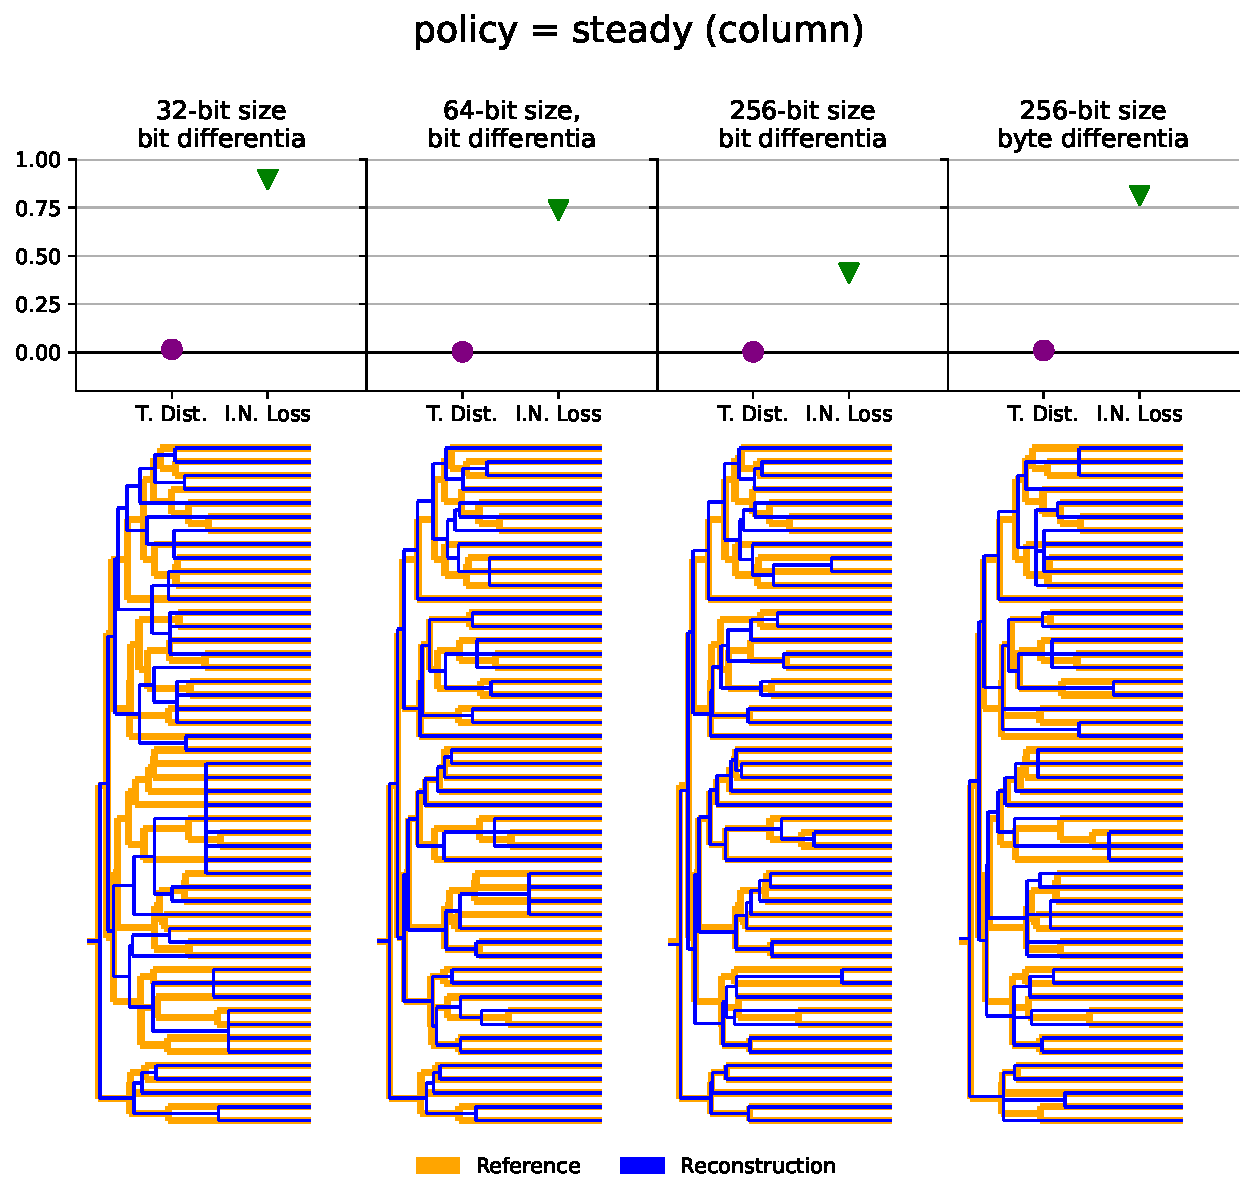
\includegraphics[width=0.5\textwidth]{binder/binder/outplots/a=examplepanel+policy=col-steady+regime=drift+ext=}%
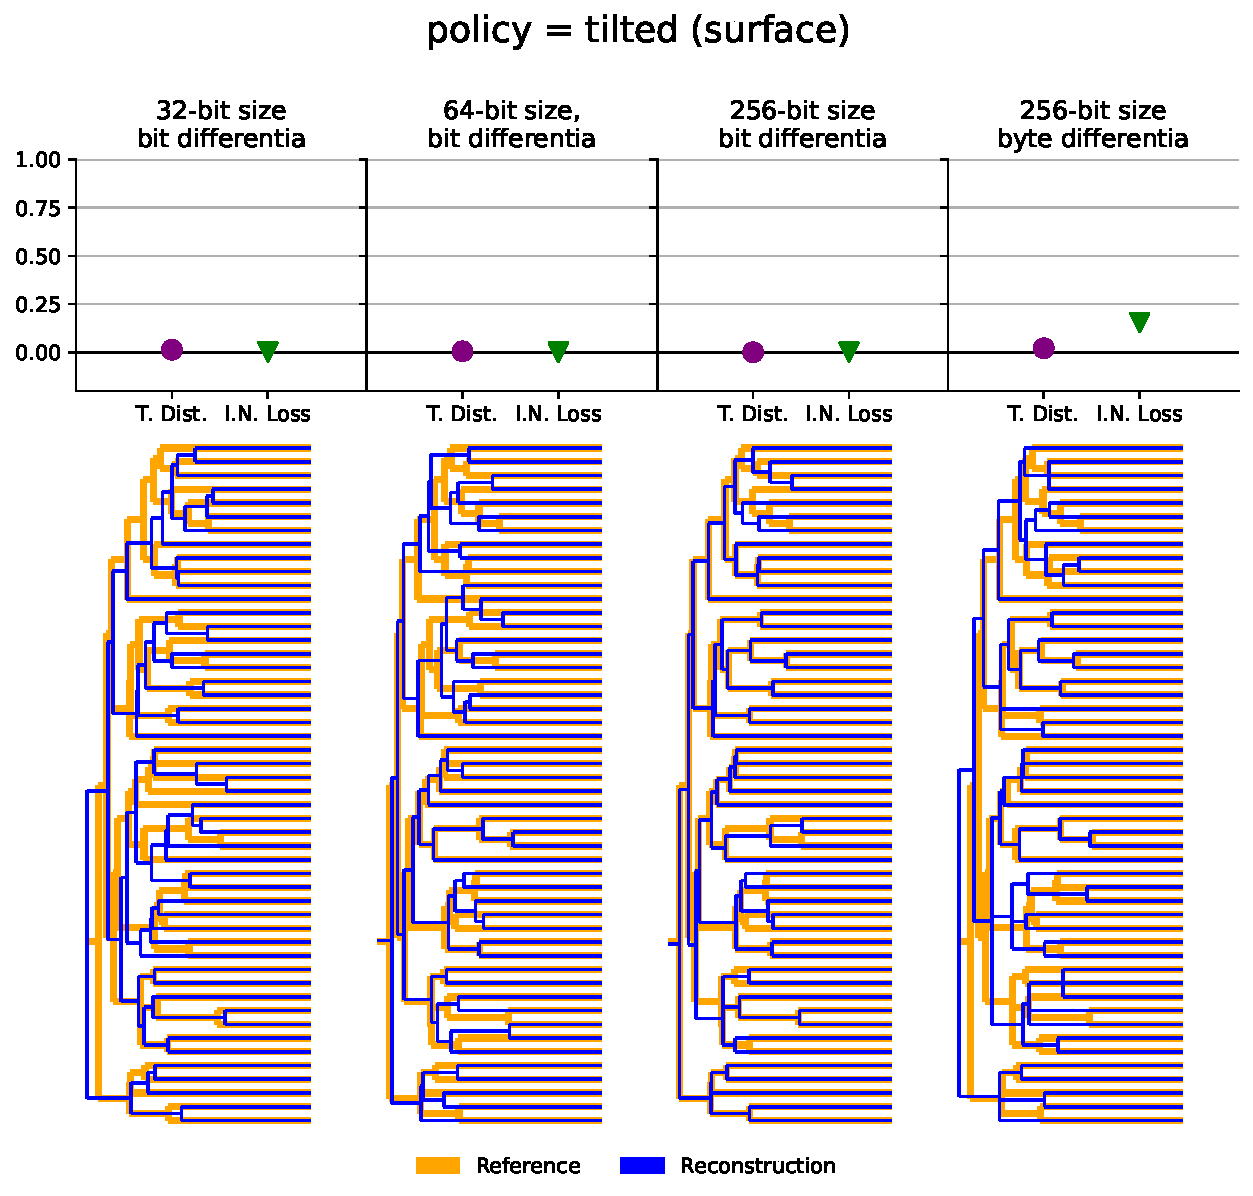
\includegraphics[width=0.5\textwidth]{binder/binder/outplots/a=examplepanel+policy=surf-tilted+regime=drift+ext=}
\caption{drift regime --- high phylogenetic richness}
\label{fig:examplepanel-drift}
\end{subfigure}

\begin{subfigure}[b]{\textwidth}
\centering
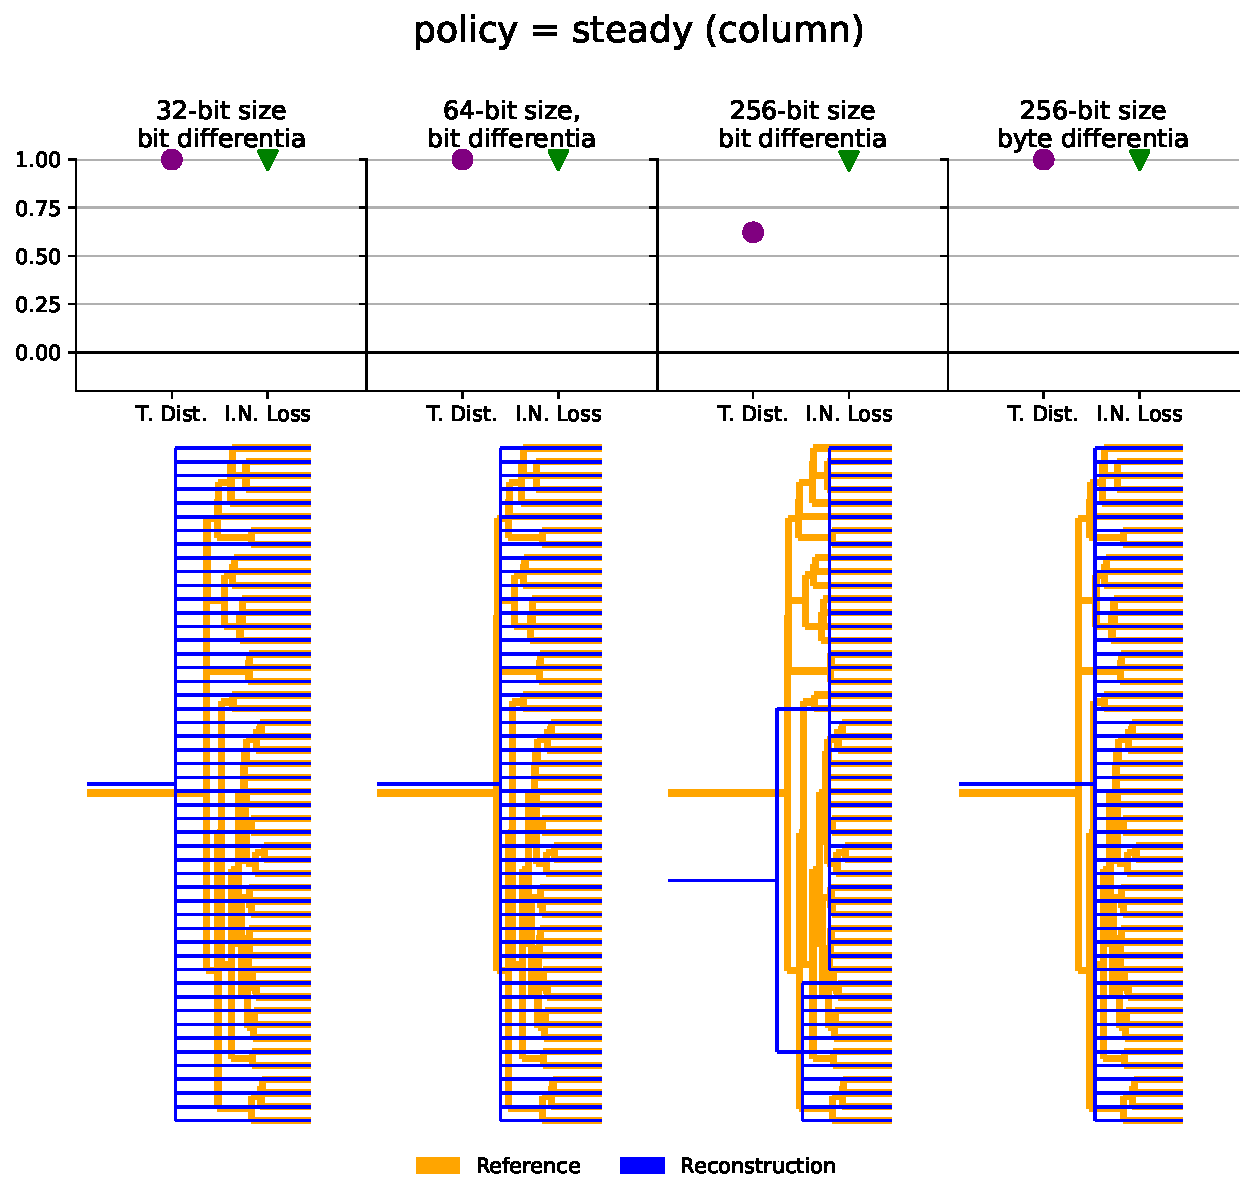
\includegraphics[width=0.5\textwidth]{binder/binder/outplots/a=examplepanel+policy=col-steady+regime=plain+ext=}%
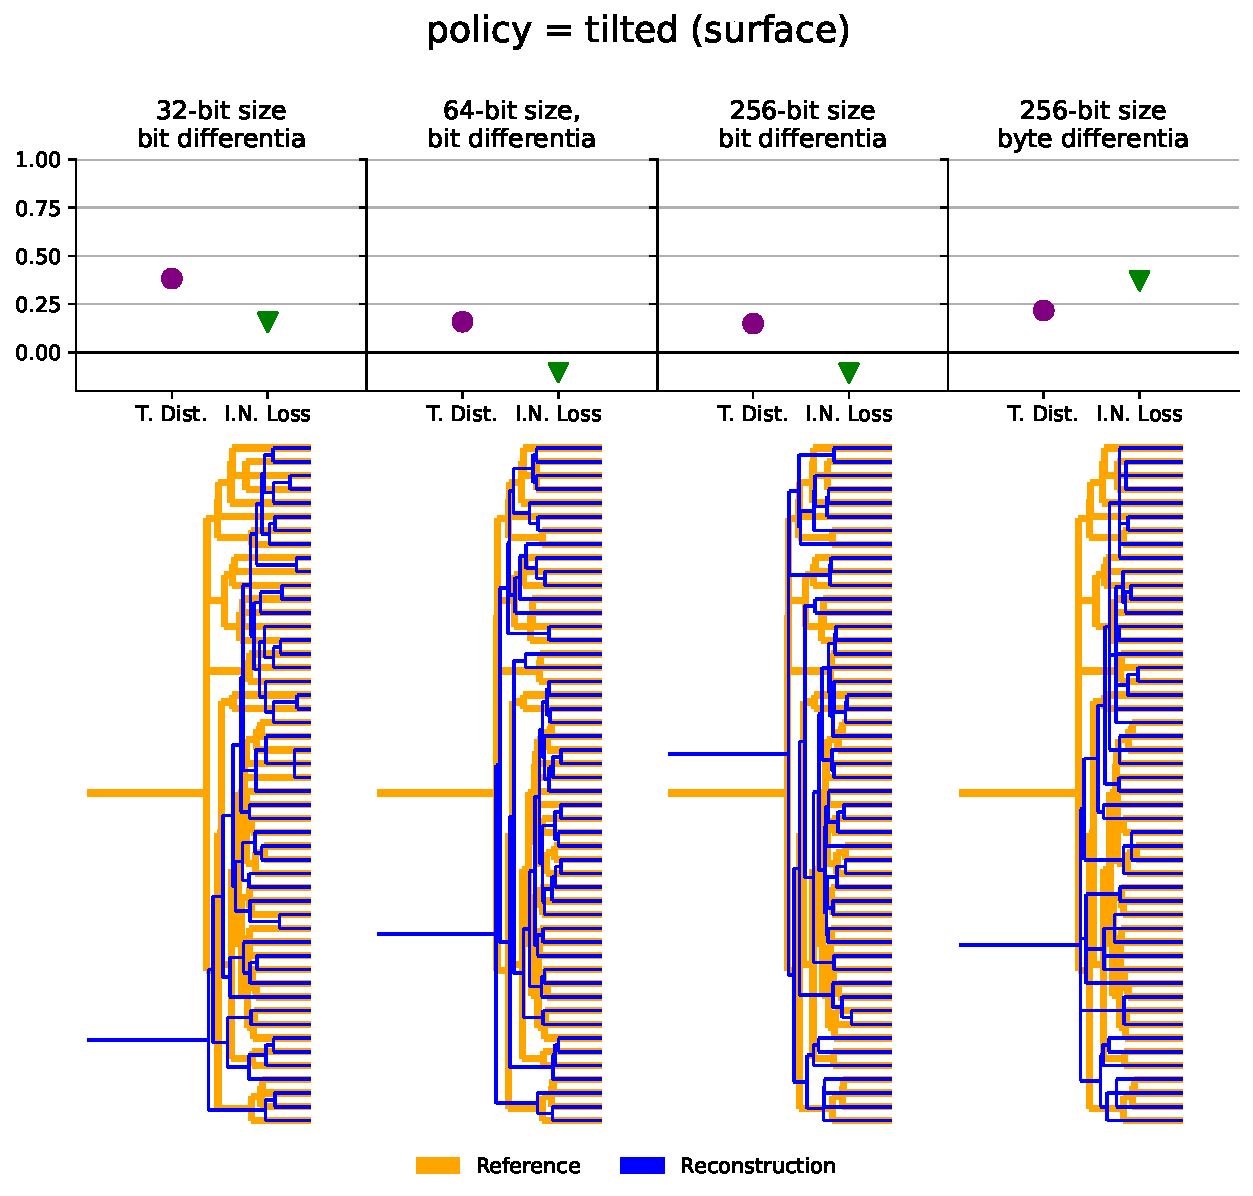
\includegraphics[width=0.5\textwidth]{binder/binder/outplots/a=examplepanel+policy=surf-tilted+regime=plain+ext=}
\caption{plain regime --- low phylogenetic richness}
\label{fig:examplepanel-plain}
\end{subfigure}

  \caption{%
  \textbf{Reconstruction vs. Reference Examples.}
  Comparison of reconstruction to reference tree for steady and tilted policies under drift (\ref{fig:examplepanel-drift}) and plain (\ref{fig:examplepanel-plain}) evolutionary regimes.
  Panel tops show reconstruction quality metrics and panel bottoms overlay reconstruction (blue) on reference tree (orange). 
  Phylogeny time axes are log scale.
  Note that overlay layout is naive, so can underrepresent agreement between trees; however, comparison is informative to general differences in tree structure.
  }
  \label{fig:examplepanel}

\end{figure*}
